%&format -translate-file pdf
\documentclass{article}
\usepackage{graphicx}
\usepackage{listings}
\lstset{basicstyle=\ttfamily\tiny}
\title{Project 1}
\author{RT Hatfield}
\date{13 September 2016}
\begin{document}
\maketitle
\begin{itemize}
    \item See Figure 1.
    \begin{figure}[p]
        \centering
        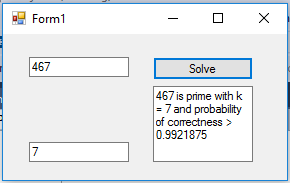
\includegraphics[resolution=144]{project1}
        \caption{Screenshot in action}
    \end{figure}
    \item 
    \begin{lstlisting}
public partial class Form1 : Form
{
    public Form1()
    {
        InitializeComponent();
    }

    private void button_Click(object sender, EventArgs e)
    {
        long k = 5; 
        if (! k_hole.Text.Contains("k"))
        {
            k = Convert.ToInt64(k_hole.Text);
        }
        if (prime_test(Convert.ToInt64(input.Text), k)) \\ call actual primality tester
        {
            output.Text = input.Text + " is prime with k = " + k.ToString() 
                    + " and probability of correctness > " + (1 - (1 / Math.Pow(2, k))).ToString();
        }
        else
        {
            output.Text = input.Text + " is NOT prime with k = " + k.ToString();
        }
    }

    private bool prime_test(long N, long k)
    {
        ISet < long > a = new HashSet<long>();
        Random rand = new Random();

        for (int i = 0; i < k; i++) // complexity O(k)
        {
            long t = rand.Next((int) N);
            if (a.Contains(t)) // we already used this random number, try again
            {
                i--;
            }
            else
            {
                a.Add(t);   // remember this number
                if(modexp(t, N - 1, N) != 1) // primality test
                {
                    return false;   // if any ONE draw does not test positive, we reject N as non-prime
                }
            }
        }
        return true;  // done k tests, all positive: N is prime
    }

    long modexp(long x, long y, long N) // modular exponentiation, O(n^3)
    {
        if (y == 0) // base case
        {
            return 1;
        }
        if (y % 2 == 0) // this if-else simulates a floor function, as well as giving us the odd and even cases
        {
            long z = modexp(x, y / 2, N); // if y is even, floor is just half
            return  (z * z) % N;
        }
        else
        {
            long z = modexp(x, (y - 1) / 2, N); // if y is odd, floor is (y-1)/2
            return (x * (z * z)) % N;
        }
    }
}
    \end{lstlisting}
    \item The two key areas of the code are the prime tester, and the modular exponentiation function that it relies on.  Everything else is O(1) because it occurs once per run.
    The primality tester is just a loop that runs up to $k$ times, which calls the modular exponentiation loop every run.  Modular exponentiation runs in $O(n^3)$, where $n$ is 
    the number of bits in the largest of $x, y$ and $N$, because it will multiply two $n$-bit numbers up to $n$ times.  \lstinline'long's are 64 bits in C\#, so at most this 
    particular piece of code will involve 262,144 stack frames.  Ultimately, the primality tester is in the $O(kn^3) = O(n^3)$ complexity class.
    \item The probability of correctness is determined by the formula on page 35 of the textbook.  This is really the sum of the independent probability that any one iteration
    of the primality test gives a false positive, which is $\frac{1}{2}$.  Independent probabilities are summed by multiplying, so the total probability of a false positive 
    during $k$ iterations is $\frac{1}{2^k}$.
\end{itemize}
\end{document}